% Options for packages loaded elsewhere
\PassOptionsToPackage{unicode}{hyperref}
\PassOptionsToPackage{hyphens}{url}
%
\documentclass[
]{article}
\usepackage{amsmath,amssymb}
\usepackage{ctex}
\usepackage{iftex}
\ifPDFTeX
  \usepackage[T1]{fontenc}
  \usepackage[utf8]{inputenc}
  \usepackage{textcomp} % provide euro and other symbols
\else % if luatex or xetex
  \usepackage{unicode-math} % this also loads fontspec
  \defaultfontfeatures{Scale=MatchLowercase}
  \defaultfontfeatures[\rmfamily]{Ligatures=TeX,Scale=1}
\fi
\usepackage{lmodern}
\ifPDFTeX\else
  % xetex/luatex font selection
\fi
% Use upquote if available, for straight quotes in verbatim environments
\IfFileExists{upquote.sty}{\usepackage{upquote}}{}
\IfFileExists{microtype.sty}{% use microtype if available
  \usepackage[]{microtype}
  \UseMicrotypeSet[protrusion]{basicmath} % disable protrusion for tt fonts
}{}
\makeatletter
\@ifundefined{KOMAClassName}{% if non-KOMA class
  \IfFileExists{parskip.sty}{%
    \usepackage{parskip}
  }{% else
    \setlength{\parindent}{0pt}
    \setlength{\parskip}{6pt plus 2pt minus 1pt}}
}{% if KOMA class
  \KOMAoptions{parskip=half}}
\makeatother
\usepackage{xcolor}
\usepackage{color}
\usepackage{fancyvrb}
\newcommand{\VerbBar}{|}
\newcommand{\VERB}{\Verb[commandchars=\\\{\}]}
\DefineVerbatimEnvironment{Highlighting}{Verbatim}{commandchars=\\\{\}}
% Add ',fontsize=\small' for more characters per line
\newenvironment{Shaded}{}{}
\newcommand{\AlertTok}[1]{\textcolor[rgb]{1.00,0.00,0.00}{\textbf{#1}}}
\newcommand{\AnnotationTok}[1]{\textcolor[rgb]{0.38,0.63,0.69}{\textbf{\textit{#1}}}}
\newcommand{\AttributeTok}[1]{\textcolor[rgb]{0.49,0.56,0.16}{#1}}
\newcommand{\BaseNTok}[1]{\textcolor[rgb]{0.25,0.63,0.44}{#1}}
\newcommand{\BuiltInTok}[1]{\textcolor[rgb]{0.00,0.50,0.00}{#1}}
\newcommand{\CharTok}[1]{\textcolor[rgb]{0.25,0.44,0.63}{#1}}
\newcommand{\CommentTok}[1]{\textcolor[rgb]{0.38,0.63,0.69}{\textit{#1}}}
\newcommand{\CommentVarTok}[1]{\textcolor[rgb]{0.38,0.63,0.69}{\textbf{\textit{#1}}}}
\newcommand{\ConstantTok}[1]{\textcolor[rgb]{0.53,0.00,0.00}{#1}}
\newcommand{\ControlFlowTok}[1]{\textcolor[rgb]{0.00,0.44,0.13}{\textbf{#1}}}
\newcommand{\DataTypeTok}[1]{\textcolor[rgb]{0.56,0.13,0.00}{#1}}
\newcommand{\DecValTok}[1]{\textcolor[rgb]{0.25,0.63,0.44}{#1}}
\newcommand{\DocumentationTok}[1]{\textcolor[rgb]{0.73,0.13,0.13}{\textit{#1}}}
\newcommand{\ErrorTok}[1]{\textcolor[rgb]{1.00,0.00,0.00}{\textbf{#1}}}
\newcommand{\ExtensionTok}[1]{#1}
\newcommand{\FloatTok}[1]{\textcolor[rgb]{0.25,0.63,0.44}{#1}}
\newcommand{\FunctionTok}[1]{\textcolor[rgb]{0.02,0.16,0.49}{#1}}
\newcommand{\ImportTok}[1]{\textcolor[rgb]{0.00,0.50,0.00}{\textbf{#1}}}
\newcommand{\InformationTok}[1]{\textcolor[rgb]{0.38,0.63,0.69}{\textbf{\textit{#1}}}}
\newcommand{\KeywordTok}[1]{\textcolor[rgb]{0.00,0.44,0.13}{\textbf{#1}}}
\newcommand{\NormalTok}[1]{#1}
\newcommand{\OperatorTok}[1]{\textcolor[rgb]{0.40,0.40,0.40}{#1}}
\newcommand{\OtherTok}[1]{\textcolor[rgb]{0.00,0.44,0.13}{#1}}
\newcommand{\PreprocessorTok}[1]{\textcolor[rgb]{0.74,0.48,0.00}{#1}}
\newcommand{\RegionMarkerTok}[1]{#1}
\newcommand{\SpecialCharTok}[1]{\textcolor[rgb]{0.25,0.44,0.63}{#1}}
\newcommand{\SpecialStringTok}[1]{\textcolor[rgb]{0.73,0.40,0.53}{#1}}
\newcommand{\StringTok}[1]{\textcolor[rgb]{0.25,0.44,0.63}{#1}}
\newcommand{\VariableTok}[1]{\textcolor[rgb]{0.10,0.09,0.49}{#1}}
\newcommand{\VerbatimStringTok}[1]{\textcolor[rgb]{0.25,0.44,0.63}{#1}}
\newcommand{\WarningTok}[1]{\textcolor[rgb]{0.38,0.63,0.69}{\textbf{\textit{#1}}}}
\usepackage{graphicx}
\makeatletter
\def\maxwidth{\ifdim\Gin@nat@width>\linewidth\linewidth\else\Gin@nat@width\fi}
\def\maxheight{\ifdim\Gin@nat@height>\textheight\textheight\else\Gin@nat@height\fi}
\makeatother
% Scale images if necessary, so that they will not overflow the page
% margins by default, and it is still possible to overwrite the defaults
% using explicit options in \includegraphics[width, height, ...]{}
\setkeys{Gin}{width=\maxwidth,height=\maxheight,keepaspectratio}
% Set default figure placement to htbp
\makeatletter
\def\fps@figure{htbp}
\makeatother
\setlength{\emergencystretch}{3em} % prevent overfull lines
\providecommand{\tightlist}{%
  \setlength{\itemsep}{0pt}\setlength{\parskip}{0pt}}
\setcounter{secnumdepth}{-\maxdimen} % remove section numbering
\ifLuaTeX
  \usepackage{selnolig}  % disable illegal ligatures
\fi
\usepackage{bookmark}
\IfFileExists{xurl.sty}{\usepackage{xurl}}{} % add URL line breaks if available
\urlstyle{same}
\hypersetup{
  hidelinks,
  pdfcreator={LaTeX via pandoc}}

\author{}
\date{}

\begin{document}

\section{项目进展状况小结}\label{ux9879ux76eeux8fdbux5c55ux72b6ux51b5ux5c0fux7ed3}

\subsection{目标回顾}\label{ux76eeux6807ux56deux987e}

根据任务书,我们计划于4月前完成项目目标确立和创新点选取,研究方法和技术选择,并基于选择的技术路线完成训练数据集的搭建。

目前,我们已经明确了项目目标:比较基于抽象语法树(AST)的CodeBERT,基于数据流图(DFG)的GraphCodeBert和同时训练代码处理和自然语言处理的UniXcoder这三种预训练模型在源代码缺陷定位任务上的表现。我们的创新点在于,此前还没有研究关注最新的NL-PL双模态大模型在错误定位(Fault-localization)上的应用。

我们的选择的技术路线类似传统的基于信息检索(IR-based)的错误定位,研究方法类似自然语言处理领域常用的预训练+微调模式。

数据集方面,我们原先计划通过爬虫获取Github错误报告的形式构建,但在研究的过程中,我们发现大型开源项目往往会使用类似Bugzilla的错误跟踪系统,我们只需要调用对应的api就可以获取完整的错误报告。此外,为了与IRBL领域其他研究进行横向对比,我们需要选择更为通用的数据集。因此,我们从此前研究常用的数据集出发,构建了一个基于错误跟踪系统的数据集,并已经完成了训练数据的预处理。此外,我们选择的预训练模型已经在CodeSearchNet代码搜索数据集上进行了预训练,并可以针对特定编程语言进行进一步迁移训练。我们计划把该数据集中的Java语言代码搜索数据集与我们此前构建的Java语言错误报告数据集进行混合,但目前还没有完成两种数据集格式的统一。

模型选择方面,我们明确分工,由3名组员分别去阅读3个模型对应的代码。

此外,为了完成后续预训练模型的迁移训练,我们申请了东南大学大数据共享平台账号,并使用云计算节点完成了训练数据集的预处理(使用云CPU),并尝试使用云GPU对预训练模型进行迁移训练。训练结果如图所示,其中灰色的线是在云服务器上训练时,损失率随着训练轮数的变化曲线,其他线是在本机上用很小的模拟数据集测试代码时的结果,可以看到随着训练轮数的增加,损失函数的值呈收敛趋势。

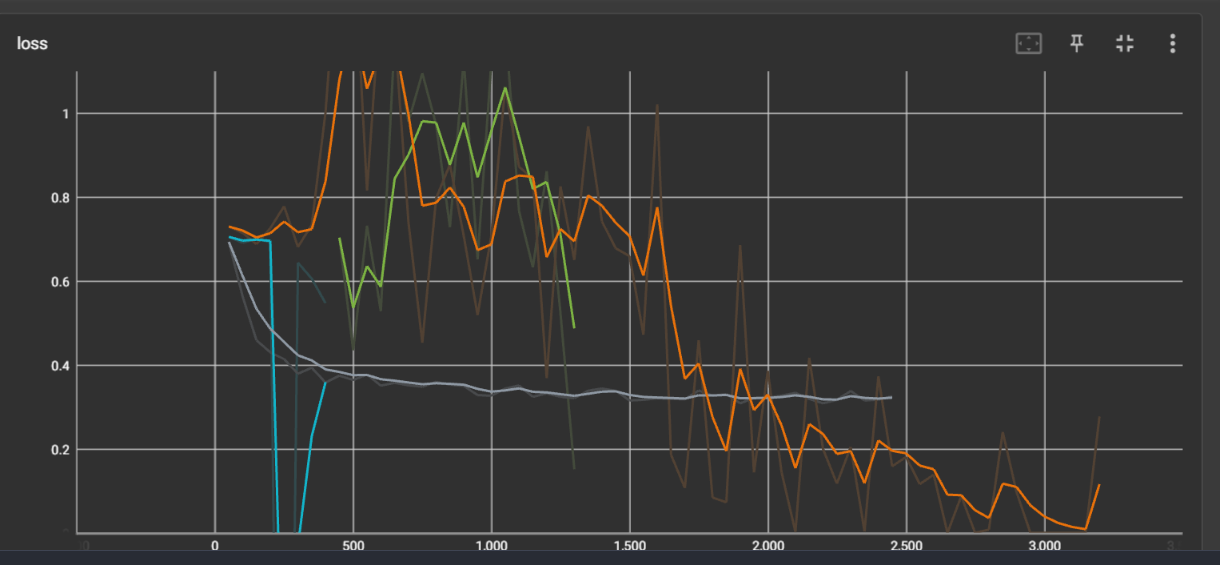
\includegraphics{D:/University/Grade2-3/Others/srtp/中期答辩/2. 前期项目研究总结/前期项目研究总结.assets/损失率曲线-1712455081776-2-1712455100425-4.png}

最后,在研究的过程中,我们共同完成了一篇针对IRFL技术和Deep-learning技术的综述报告,报告在附件中。

\subsection{数据集获取}\label{ux6570ux636eux96c6ux83b7ux53d6}

\subsubsection{前言}\label{ux524dux8a00}

数据集获取是本项目的重要组成部分,是复现模型、改进模型的前提和基础。在项目的前中期,我们已经完成了数据集选取和预处理,以及数据集的分析等任务。下面,本总结将从数据集选取、数据集处理和数据集分析三个方面来阐述本项目在数据集方面前中期的进展。

\subsubsection{数据集选取}\label{ux6570ux636eux96c6ux9009ux53d6}

\begin{enumerate}
  \def\labelenumi{\arabic{enumi}.}
  \item
        网络爬虫获取数据集的局限性

        在项目进行之初,我们计划使用python爬虫爬取Github开源项目的错误报告来搭建数据集。经过尝试,我们发现网络爬虫无法精确获取项目修改前后的代码,也就是说,我们无法找到错误报告与错误代码的对应关系;并且,爬虫所获得的数据格式与模型所需要的格式有很大的差异,处理起来非常繁琐。因此,我们选择BugLocator项目在测试中所选用的数据集。
  \item
        选择BugLocator数据集的原因

        BugLocator数据集通常被各种最先进的算法使用,并且数据集里的数据可以在Bug
        Center里找到;此外,该数据集的数据全面,包含错误的自然语言描述、修改前后的错误代码、项目作者和错误代码提交记录等信息;最后,该数据集的格式与我们将要训练的模型所需要的格式相符。
  \item
        BugLocator数据集基本介绍

        该数据集的错误报告来自AspectJ、Birt、Eclipse、JDT、SWT、Tomcat六个java开发平台,共有593个详细的错误报告。
\end{enumerate}

\subsubsection{数据集处理}\label{ux6570ux636eux96c6ux5904ux7406}

原始数据集是xml格式的,仅包含错误描述,提交时间和错误文件路径等信息,并不包含错误源代码。

以下这个函数来根据文件路径获取修改前后的代码内容。

\begin{Shaded}
  \begin{Highlighting}[]
    \KeywordTok{def}\NormalTok{ retrieve\_diff\_on\_filepath(repository, commit, filepath):}
    \NormalTok{    cmd }\OperatorTok{=} \StringTok{\textquotesingle{}git {-}C \textquotesingle{}} \OperatorTok{+}\NormalTok{ repository }\OperatorTok{+} \StringTok{\textquotesingle{} diff {-}{-}unified=0 {-}{-}no{-}prefix \textquotesingle{}} \OperatorTok{+}\NormalTok{ commit }\OperatorTok{+} \StringTok{\textquotesingle{}\^{} \textquotesingle{}} \OperatorTok{+}\NormalTok{ commit }\OperatorTok{+} \StringTok{\textquotesingle{} {-}{-} \textquotesingle{}} \OperatorTok{+}\NormalTok{ filepath}
    \NormalTok{    diff\_lines }\OperatorTok{=}\NormalTok{ subprocess.Popen(cmd, shell}\OperatorTok{=}\VariableTok{True}\NormalTok{, stdout}\OperatorTok{=}\NormalTok{subprocess.PIPE).stdout.read().decode(}\StringTok{\textquotesingle{}latin{-}1\textquotesingle{}}\NormalTok{)}
    \ControlFlowTok{return}\NormalTok{ diff\_lines}
  \end{Highlighting}
\end{Shaded}

它通过subprocess.Popen创建子进程执行git命令来获取错误代码修改前后的内容。

以下这段代码用来获取数据集中所有有修改的代码,并通过
``文件路径:代码内容'' 的字典方式存储。

\begin{Shaded}
  \begin{Highlighting}[]
    \KeywordTok{def}\NormalTok{ retrieve\_diff(repository, commit, ext}\OperatorTok{=}\StringTok{\textquotesingle{}.java\textquotesingle{}}\NormalTok{):}
    \NormalTok{    cmd }\OperatorTok{=} \StringTok{\textquotesingle{}git {-}C \textquotesingle{}} \OperatorTok{+}\NormalTok{ repository }\OperatorTok{+} \StringTok{\textquotesingle{} diff{-}tree {-}{-}no{-}commit{-}id {-}{-}name{-}only {-}r \textquotesingle{}} \OperatorTok{+}\NormalTok{ commit}
    \NormalTok{    files }\OperatorTok{=}\NormalTok{ \{\}}
    \NormalTok{    diff\_tree\_lines }\OperatorTok{=}\NormalTok{ subprocess.Popen(cmd, shell}\OperatorTok{=}\VariableTok{True}\NormalTok{, stdout}\OperatorTok{=}\NormalTok{subprocess.PIPE).stdout.read().decode(}\StringTok{\textquotesingle{}latin{-}1\textquotesingle{}}\NormalTok{).split(}\StringTok{\textquotesingle{}}\CharTok{\textbackslash{}n}\StringTok{\textquotesingle{}}\NormalTok{)}
    \ControlFlowTok{for}\NormalTok{ line }\KeywordTok{in} \BuiltInTok{iter}\NormalTok{(diff\_tree\_lines):}
    \NormalTok{        filepath }\OperatorTok{=}\NormalTok{ line.rstrip()}
    \ControlFlowTok{if}\NormalTok{ filepath }\OperatorTok{!=} \StringTok{\textquotesingle{}\textquotesingle{}} \KeywordTok{and}\NormalTok{ filepath.endswith(ext):}
    \NormalTok{            files[filepath] }\OperatorTok{=}\NormalTok{ retrieve\_diff\_on\_filepath(repository, commit, filepath)}
    \ControlFlowTok{return}\NormalTok{ files}
  \end{Highlighting}
\end{Shaded}

它先是通过创建子进程运行git命令的方式获取所有有过修改的文件的路径,再遍历这些文件路径,调用上一个函数获取每个文件中有修改的代码,最后将文件路径和相应代码以键值对的形式保存。

这段代码依然是通过创建进程运行git命令的方式获取作者、日期等信息。

\begin{Shaded}
  \begin{Highlighting}[]
    \KeywordTok{def}\NormalTok{ retrieve\_metadata(repository, commit):
    }
    \NormalTok{    full\_sha }\OperatorTok{=}\NormalTok{ None
    }
    \NormalTok{    author }\OperatorTok{=}\NormalTok{ None
    }
    \NormalTok{    date }\OperatorTok{=}\NormalTok{ None
    }
    \NormalTok{    message }\OperatorTok{=} \StringTok{\textquotesingle{}\textquotesingle{}}

    \NormalTok{    cmd }\OperatorTok{=} \StringTok{\textquotesingle{}git {-}C \textquotesingle{}} \OperatorTok{+}\NormalTok{ repository }\OperatorTok{+} \StringTok{\textquotesingle{} show {-}s \textquotesingle{}} \OperatorTok{+}\NormalTok{ commit
    }
    \NormalTok{    show\_lines }\OperatorTok{=}\NormalTok{ subprocess.Popen(cmd, shell}\OperatorTok{=}\VariableTok{True}\NormalTok{, stdout}\OperatorTok{=}\NormalTok{subprocess.PIPE).stdout.read().decode(}\StringTok{\textquotesingle{}latin{-}1\textquotesingle{}}\NormalTok{).split(}\StringTok{\textquotesingle{}}\CharTok{\textbackslash{}n}\StringTok{\textquotesingle{}}\NormalTok{)
    }
    \ControlFlowTok{for}\NormalTok{ index, line }\KeywordTok{in} \BuiltInTok{enumerate}\NormalTok{(show\_lines):
    }
    \ControlFlowTok{if}\NormalTok{ index }\OperatorTok{==} \DecValTok{0}\NormalTok{:
    }
    \NormalTok{            full\_sha }\OperatorTok{=}\NormalTok{ line
    }
    \ControlFlowTok{elif}\NormalTok{ index }\OperatorTok{==} \DecValTok{1}\NormalTok{:
    }
    \NormalTok{            author }\OperatorTok{=}\NormalTok{ line
    }
    \ControlFlowTok{elif}\NormalTok{ index }\OperatorTok{==} \DecValTok{2}\NormalTok{:
    }
    \NormalTok{            date }\OperatorTok{=}\NormalTok{ line
    }
    \ControlFlowTok{else}\NormalTok{:
    }
    \NormalTok{            message }\OperatorTok{+=}\NormalTok{ line
    }
    \NormalTok{    metadata }\OperatorTok{=}\NormalTok{ \{}\StringTok{\textquotesingle{}sha\textquotesingle{}}\NormalTok{: full\_sha, }\StringTok{\textquotesingle{}author\textquotesingle{}}\NormalTok{: author, }\StringTok{\textquotesingle{}date\textquotesingle{}}\NormalTok{: date, }\StringTok{\textquotesingle{}message\textquotesingle{}}\NormalTok{: message\}
    }
    \ControlFlowTok{return}\NormalTok{ metadata}
  \end{Highlighting}
\end{Shaded}

将数据集转变为json格式,获取json文件。

\begin{Shaded}
  \begin{Highlighting}[]
    \KeywordTok{def}\NormalTok{ main():}
    \NormalTok{    bug\_reports\_file }\OperatorTok{=}\NormalTok{ sys.argv[}\DecValTok{1}\NormalTok{]}
    \NormalTok{    repository }\OperatorTok{=}\NormalTok{ sys.argv[}\DecValTok{2}\NormalTok{]}
    \NormalTok{    json\_file\_name }\OperatorTok{=}\NormalTok{ sys.argv[}\DecValTok{3}\NormalTok{]}
    \NormalTok{    dataset }\OperatorTok{=}\NormalTok{ load\_dataset(bug\_reports\_file, repository)}
    \ControlFlowTok{with} \BuiltInTok{open}\NormalTok{(json\_file\_name, }\StringTok{\textquotesingle{}w\textquotesingle{}}\NormalTok{) }\ImportTok{as}\NormalTok{ f:}
    \NormalTok{        dump(dataset, f)}
  \end{Highlighting}
\end{Shaded}

\subsubsection{数据集分析}\label{ux6570ux636eux96c6ux5206ux6790}

这是一个处理好了的数据集个体实例

\begin{enumerate}
  \def\labelenumi{\arabic{enumi}.}
  \item
        `bug\_report'部分:
\end{enumerate}

\begin{Shaded}
  \begin{Highlighting}[]
    \ErrorTok{"bug\_id":} \ErrorTok{"111915",}
    \ErrorTok{"status":} \ErrorTok{"resolved} \ErrorTok{fixed",}
    \ErrorTok{"result":} \ErrorTok{"7:/aspectj/systemtest/ajc150/Ajc150Tests.java\textbackslash{}n} \ErrorTok{12:/aspectj/weaver/patterns/ReferencePointcut.java",}
    \ErrorTok{"timestamp":} \ErrorTok{"1128700000",}
    \ErrorTok{"commit":} \ErrorTok{"3021284",}
    \ErrorTok{"description":} \ErrorTok{"BCException} \ErrorTok{thrown:} \ErrorTok{illegal} \ErrorTok{change} \ErrorTok{to} \ErrorTok{pointcut} \ErrorTok{\#Files=11",}
    \ErrorTok{"id":} \ErrorTok{"335",}
    \ErrorTok{"summary":} \ErrorTok{"Bug} \ErrorTok{111915}  \ErrorTok{illegal} \ErrorTok{change} \ErrorTok{to} \ErrorTok{pointcut} \ErrorTok{declaration",}
    \ErrorTok{"preceding\_commit":} \ErrorTok{"bba983e0afce48d09316b46a72dbe6d2ae4c14b4",}
  \end{Highlighting}
\end{Shaded}

这个很长的\textquotesingle description\textquotesingle 指的是错误具体发生的位置;

\textquotesingle summary\textquotesingle 就是对错误的自然语言描述:''Bug
111915 illegal change to pointcut
declaration``,表示的错误是''切入点声明的非法更改``。

\begin{enumerate}
  \def\labelenumi{\arabic{enumi}.}
  \item
        `commit'部分:
\end{enumerate}

\begin{Shaded}
  \begin{Highlighting}[]
    \ErrorTok{"diff":} \FunctionTok{\{}
    \ErrorTok{tests/src/org/aspectj/systemtest/ajc150/Ajc150Tests.java}\FunctionTok{:}
    \ErrorTok{diff} \ErrorTok{{-}{-}git} \ErrorTok{tests/src/org/aspectj/systemtest/ajc150/Ajc150Tests.java} \ErrorTok{tests/src/org/aspectj/systemtest/ajc150/Ajc150Tests.java}
    \ErrorTok{index} \ErrorTok{a6f8acb461..}\DecValTok{1}\ErrorTok{aabffea64} \DecValTok{100644}
    \ErrorTok{{-}{-}{-}} \ErrorTok{tests/src/org/aspectj/systemtest/ajc150/Ajc150Tests.java}
    \ErrorTok{+++} \ErrorTok{tests/src/org/aspectj/systemtest/ajc150/Ajc150Tests.java}
    \ErrorTok{@@} \DecValTok{{-}487}\FunctionTok{,}\ErrorTok{0} \ErrorTok{+488}\FunctionTok{,}\ErrorTok{4} \ErrorTok{@@} \ErrorTok{public} \ErrorTok{class} \ErrorTok{Ajc150Tests} \ErrorTok{extends} \ErrorTok{org.aspectj.testing.XMLBasedAjcTestCase} \ErrorTok{\{}
    \ErrorTok{+}  \ErrorTok{public} \ErrorTok{void} \ErrorTok{testIllegalChangeToPointcutDeclaration\_pr111915()} \ErrorTok{\{}
    \ErrorTok{+}	\ErrorTok{runTest(}\DataTypeTok{"test illegal change to pointcut declaration"}\ErrorTok{);}
    \ErrorTok{+}  \FunctionTok{\}}

    \ErrorTok{"metadata":} \FunctionTok{\{}
    \DataTypeTok{"date"}\FunctionTok{:} \StringTok{"Fri Oct 21 06:56:11 2005 +0000"}\FunctionTok{,}
    \DataTypeTok{"sha"}\FunctionTok{:} \StringTok{"3021284f5d910a406d26a01ce836bbb5f5cd6bfc"}\FunctionTok{,}
    \DataTypeTok{"message"}\FunctionTok{:} \StringTok{"test and fix for pr111915"}\FunctionTok{,}
    \DataTypeTok{"author"}\FunctionTok{:} \StringTok{"aclement \textless{}aclement\textgreater{}"}\FunctionTok{,}
    \DataTypeTok{"timestamp"}\FunctionTok{:} \FloatTok{1129877771.0}
    \FunctionTok{\}}\ErrorTok{,}
  \end{Highlighting}
\end{Shaded}

`diff'部分的

\begin{Shaded}
  \begin{Highlighting}[]
    \ErrorTok{tests/src/org/aspectj/systemtest/ajc150/Ajc150Tests.java:}
  \end{Highlighting}
\end{Shaded}

即为错误代码所在路径,对应的

\begin{Shaded}
  \begin{Highlighting}[]
    \ErrorTok{+}  \ErrorTok{public} \ErrorTok{void} \ErrorTok{testIllegalChangeToPointcutDeclaration\_pr111915()} \FunctionTok{\{}
    \ErrorTok{+}	\ErrorTok{runTest(}\DataTypeTok{"test illegal change to pointcut declaration"}\ErrorTok{);}
    \ErrorTok{+}  \FunctionTok{\}}
  \end{Highlighting}
\end{Shaded}

为错误源代码。(该部分还有三个同样格式的路径、代码键值对,受篇幅限制舍去)

`metadata\textquotesingle 部分存储了作者、日期、时间等信息。

'view`部分:

\begin{Shaded}
  \begin{Highlighting}[]
    \NormalTok{\textquotesingle{}bug\_fixing\textquotesingle{}:\{}
    \NormalTok{"tests/bugs150/pr109042.aj": \{}
    \NormalTok{  "recency\_timedelta[s]": 2511442,}
    \NormalTok{  "recency[30{-}day months]": 1.0,}
    \NormalTok{  "frequency": 1,}
    \NormalTok{  "br": ["08d6a5d"]}
    \NormalTok{\}}
    \NormalTok{\}}
    \NormalTok{(还有897个相同结构,此处省去)}
  \end{Highlighting}
\end{Shaded}

该部分记录错误代码的提交记录。

\subsubsection{总结}\label{ux603bux7ed3}

我们在项目前中期搭建完成的数据集是以json的格式存储的,包含错误报告、错误代码、作者和提交记录的详细信息。

\subsection{预训练模型选择}\label{ux9884ux8badux7ec3ux6a21ux578bux9009ux62e9}

\subsubsection{\texorpdfstring{\texttt{codeBERT}模型}{codeBERT模型}}\label{codebertux6a21ux578b}

\subsubsection{\texorpdfstring{\texttt{GraphCodeBert}模型}{GraphCodeBert模型}}\label{graphcodebertux6a21ux578b}

GraphCodeBERT模型没有考虑抽象语法树,而是采用了DFG(数据流向图)。数据流向图是一个有向图,代表了每个变量的值从哪里来到哪里去的关系。

为了显示GraphCodeBERT的有效性,作者进行了四项下游任务,包括了代码搜索、克隆检测、代码翻译和代码改错。而我们所需要的是对源代码的定位,故侧重于代码搜索。\footnote{GRAPHCODEBERT:
  PRE-TRAINING CODE REPRESENTATIONS WITH DATA FLOW (Published as a
  conference paper at ICLR 2021)}

代码搜索的任务是通过输入一段自然语言描述,模型输出从代码库中选出一段最符合描述的代码。

该模型首先按照下列方式将过滤数据集以提高质量(\(utils.py\))

\begin{itemize}
  \item
        删除代码中的注释
  \item
        删除无法将代码解析为抽象语法树的示例。
  \item
        删除文档 \#tokens 为 \textless{} 3 或 \textgreater256 的示例
  \item
        删除文档包含特殊标记的示例(例如 \textless img ...\textgreater{} 或
        https:...)
  \item
        删除文档不是英文的示例。
\end{itemize}

最后经过实验发现该模型实现了最先进的性能。

该模型首先将数据集生成对应语言的DFG
(\(DFG.py\)),再将代码转换为特征,用于训练机器学习模型,最后训练模型并对模型进行评估,打印评估结果。

该模型的主要创新点便是DFG,例如:

\begin{Shaded}
  \begin{Highlighting}[]
    \KeywordTok{def}\NormalTok{ bubble\_sort(lst):}
    \CommentTok{\textquotesingle{}\textquotesingle{}\textquotesingle{}}
    \CommentTok{    Sorts a list of integers using bubble sort.}
    \CommentTok{    \textquotesingle{}\textquotesingle{}\textquotesingle{}}
    \NormalTok{    n }\OperatorTok{=} \BuiltInTok{len}\NormalTok{(lst)}
    \ControlFlowTok{for}\NormalTok{ i }\KeywordTok{in} \BuiltInTok{range}\NormalTok{(n):}
    \ControlFlowTok{for}\NormalTok{ j }\KeywordTok{in} \BuiltInTok{range}\NormalTok{(}\DecValTok{0}\NormalTok{, n}\OperatorTok{{-}}\NormalTok{i}\OperatorTok{{-}}\DecValTok{1}\NormalTok{):}
    \ControlFlowTok{if}\NormalTok{ lst[j] }\OperatorTok{\textgreater{}}\NormalTok{ lst[j}\OperatorTok{+}\DecValTok{1}\NormalTok{] :}
    \NormalTok{                lst[j], lst[j}\OperatorTok{+}\DecValTok{1}\NormalTok{] }\OperatorTok{=}\NormalTok{ lst[j}\OperatorTok{+}\DecValTok{1}\NormalTok{], lst[j]}
    \ControlFlowTok{return}\NormalTok{ lst}
  \end{Highlighting}
\end{Shaded}

经过testDemo.ipynb处理后得到数据集,我们需要的部分为original\_string和docstring\_tokens部分。

\begin{Shaded}
  \begin{Highlighting}[]
    \NormalTok{original\_string部分:}
    \KeywordTok{def}\NormalTok{ bubble\_sort(lst):\textbackslash{}n    n }\OperatorTok{=} \BuiltInTok{len}\NormalTok{(lst)\textbackslash{}n    }\ControlFlowTok{for}\NormalTok{ i }\KeywordTok{in} \BuiltInTok{range}\NormalTok{(n):\textbackslash{}n        }\ControlFlowTok{for}\NormalTok{ j }\KeywordTok{in} \BuiltInTok{range}\NormalTok{(}\DecValTok{0}\NormalTok{, n}\OperatorTok{{-}}\NormalTok{i}\OperatorTok{{-}}\DecValTok{1}\NormalTok{):\textbackslash{}n            }\ControlFlowTok{if}\NormalTok{ lst[j] }\OperatorTok{\textgreater{}}\NormalTok{ lst[j}\OperatorTok{+}\DecValTok{1}\NormalTok{] :\textbackslash{}n                lst[j], lst[j}\OperatorTok{+}\DecValTok{1}\NormalTok{] }\OperatorTok{=}\NormalTok{ lst[j}\OperatorTok{+}\DecValTok{1}\NormalTok{], lst[j]\textbackslash{}n    }\ControlFlowTok{return}\NormalTok{ lst\textbackslash{}n}

    \NormalTok{docstring\_tokens部分:}
    \NormalTok{[}\StringTok{"Sorts"}\NormalTok{, }\StringTok{"a"}\NormalTok{, }\StringTok{"list"}\NormalTok{, }\StringTok{"of"}\NormalTok{, }\StringTok{"integers"}\NormalTok{, }\StringTok{"using"}\NormalTok{, }\StringTok{"bubble"}\NormalTok{, }\StringTok{"sort"}\NormalTok{, }\StringTok{"."}\NormalTok{]}
  \end{Highlighting}
\end{Shaded}

首先逐个记录出现的变量,并用左闭右开的集合保存入dfg\_to\_code,再根据这个变量由哪些变量得到绘制出dfg\_to\_dfg

\subsubsection{Unixcoder(跨模态预训练模型)}\label{unixcoderux8de8ux6a21ux6001ux9884ux8badux7ec3ux6a21ux578buxff09}

一、模型概述

1.本模型支持与coding相关的代码理解和生成任务。

2.模型分类\\
(1)unixcoder-base-unimodal: 在 C4 和 CodeSearchNet 数据集(不含
NL)上进行预训练\\
(2)unixcoder-base: 继续在 CodeSearchNet 数据集的 NL-PL 对上预训练
unixcoder-base-unimodal。该模型可支持六种语言java、ruby、python、php、javascript
和 go。\\
(3)unixcoder-base-nine: 继续在 CodeSearchNet 数据集的 NL-PL 对和额外的
150 万个 C、C++ 和 C\# 编程语言的 NL-PL
对上预训练。该模型可支持九种语言java、ruby、python、php、javascript、go、c、c++
和 c\#。

3.安装依赖\\
pytorch库,和transformers库\\
示例代码:\\
def \emph{init}:构建 UniXcoder
模型的各个组件,并对一些属性进行初始化设置。

二、模型示例

以下部分的示例代码给出了不同模式下多个任务的零拍示例,包括代码搜索(仅编码器)、代码补全(仅解码器)、函数名称预测(编码器-解码器)、API
推荐(编码器-解码器)、代码总结(编码器-解码器)\\
(1)仅编码器\\
示例:代码搜索\\
对给定的函数字符串进行编码,并获取其对应的嵌入向量。\\
最大值函数,最小值函数,自然语言函数

\begin{Shaded}
  \begin{Highlighting}[]
    \CommentTok{\#\#\# Encode maximum function}
    \NormalTok{func }\OperatorTok{=} \StringTok{"def f(a,b): if a\textgreater{}b: return a else return b"}
    \NormalTok{tokens\_ids }\OperatorTok{=}\NormalTok{ model.tokenize([func],max\_length}\OperatorTok{=}\DecValTok{512}\NormalTok{,mode}\OperatorTok{=}\StringTok{"\textbackslash{}\textless{}encoder{-}only\textgreater{}"}\NormalTok{)}
    \NormalTok{source\_ids }\OperatorTok{=}\NormalTok{ torch.tensor(tokens\_ids).to(device)}
    \NormalTok{tokens\_embeddings,max\_func\_embedding }\OperatorTok{=}\NormalTok{ model(source\_ids)}

    \CommentTok{\#\#\# Encode minimum function}
    \NormalTok{func }\OperatorTok{=} \StringTok{"def f(a,b): if a\textless{}b: return a else return b"}
    \NormalTok{tokens\_ids }\OperatorTok{=}\NormalTok{ model.tokenize([func],max\_length}\OperatorTok{=}\DecValTok{512}\NormalTok{,mode}\OperatorTok{=}\StringTok{"\textbackslash{}\textless{}encoder{-}only\textgreater{}"}\NormalTok{)}
    \NormalTok{source\_ids }\OperatorTok{=}\NormalTok{ torch.tensor(tokens\_ids).to(device)}
    \NormalTok{tokens\_embeddings,min\_func\_embedding }\OperatorTok{=}\NormalTok{ model(source\_ids)}

    \CommentTok{\#\#\# Encode NL}
    \NormalTok{nl }\OperatorTok{=} \StringTok{"return maximum value"}
    \NormalTok{tokens\_ids }\OperatorTok{=}\NormalTok{ model.tokenize([nl],max\_length}\OperatorTok{=}\DecValTok{512}\NormalTok{,mode}\OperatorTok{=}\StringTok{"\textbackslash{}\textless{}encoder{-}only\textgreater{}"}\NormalTok{)}
    \NormalTok{source\_ids }\OperatorTok{=}\NormalTok{ torch.tensor(tokens\_ids).to(device)}
    \NormalTok{tokens\_embeddings,nl\_embedding }\OperatorTok{=}\NormalTok{ model(source\_ids)}

    \BuiltInTok{print}\NormalTok{(max\_func\_embedding.shape)}
    \BuiltInTok{print}\NormalTok{(max\_func\_embedding)}

    \CommentTok{\#\#\#\# the outcome of the print}

    \NormalTok{torch.Size([}\DecValTok{1}\NormalTok{, }\DecValTok{768}\NormalTok{])}
    \NormalTok{tensor([[ }\FloatTok{8.6533e{-}01}\NormalTok{, }\OperatorTok{{-}}\FloatTok{1.9796e+00}\NormalTok{, }\OperatorTok{{-}}\FloatTok{8.6849e{-}01}\NormalTok{,  }\FloatTok{4.2652e{-}01}\NormalTok{, }\OperatorTok{{-}}\FloatTok{5.3696e{-}01}\NormalTok{,}
    \OperatorTok{{-}}\FloatTok{1.5521e{-}01}\NormalTok{,  }\FloatTok{5.3770e{-}01}\NormalTok{,  }\FloatTok{3.4199e{-}01}\NormalTok{,  }\FloatTok{3.6305e{-}01}\NormalTok{, }\OperatorTok{{-}}\FloatTok{3.9391e{-}01}\NormalTok{,}
    \OperatorTok{{-}}\FloatTok{1.1816e+00}\NormalTok{,  }\FloatTok{2.6010e+00}\NormalTok{, }\OperatorTok{{-}}\FloatTok{7.7133e{-}01}\NormalTok{,  }\FloatTok{1.8441e+00}\NormalTok{,  }\FloatTok{2.3645e+00}\NormalTok{,}
    \NormalTok{				 ...,}
    \OperatorTok{{-}}\FloatTok{2.9188e+00}\NormalTok{,  }\FloatTok{1.2555e+00}\NormalTok{, }\OperatorTok{{-}}\FloatTok{1.9953e+00}\NormalTok{, }\OperatorTok{{-}}\FloatTok{1.9795e+00}\NormalTok{,  }\FloatTok{1.7279e+00}\NormalTok{,}
    \FloatTok{6.4590e{-}01}\NormalTok{, }\OperatorTok{{-}}\FloatTok{5.2769e{-}02}\NormalTok{,  }\FloatTok{2.4965e{-}01}\NormalTok{,  }\FloatTok{2.3962e{-}02}\NormalTok{,  }\FloatTok{5.9996e{-}02}\NormalTok{,}
    \FloatTok{2.5659e+00}\NormalTok{,  }\FloatTok{3.6533e+00}\NormalTok{,  }\FloatTok{2.0301e+00}\NormalTok{]], device}\OperatorTok{=}\StringTok{\textquotesingle{}cuda:0\textquotesingle{}}\NormalTok{,}
    \NormalTok{       grad\_fn}\OperatorTok{=}\NormalTok{\textbackslash{}}\OperatorTok{\textless{}}\NormalTok{DivBackward0}\OperatorTok{\textgreater{}}\NormalTok{)}
  \end{Highlighting}
\end{Shaded}

现在,我们计算 NL
(自然语言)和两个函数之间的余弦相似度(通过对嵌入向量归一化)。虽然两个函数的差值只是一个运算符(\textless{}
和 \textgreater),但 UniXcoder 可以将它们区分开来。

\begin{Shaded}
  \begin{Highlighting}[]
    \CommentTok{\#\#\# Normalize embedding}
    \NormalTok{norm\_max\_func\_embedding }\OperatorTok{=}\NormalTok{ torch.nn.functional.normalize(max\_func\_embedding, p}\OperatorTok{=}\DecValTok{2}\NormalTok{, dim}\OperatorTok{=}\DecValTok{1}\NormalTok{)}
    \NormalTok{norm\_min\_func\_embedding }\OperatorTok{=}\NormalTok{ torch.nn.functional.normalize(min\_func\_embedding, p}\OperatorTok{=}\DecValTok{2}\NormalTok{, dim}\OperatorTok{=}\DecValTok{1}\NormalTok{)}
    \NormalTok{norm\_nl\_embedding }\OperatorTok{=}\NormalTok{ torch.nn.functional.normalize(nl\_embedding, p}\OperatorTok{=}\DecValTok{2}\NormalTok{, dim}\OperatorTok{=}\DecValTok{1}\NormalTok{)}

    \NormalTok{max\_func\_nl\_similarity }\OperatorTok{=}\NormalTok{ torch.einsum(}\StringTok{"ac,bc{-}\textgreater{}ab"}\NormalTok{,norm\_max\_func\_embedding,norm\_nl\_embedding)}
    \NormalTok{min\_func\_nl\_similarity }\OperatorTok{=}\NormalTok{ torch.einsum(}\StringTok{"ac,bc{-}\textgreater{}ab"}\NormalTok{,norm\_min\_func\_embedding,norm\_nl\_embedding)}

    \BuiltInTok{print}\NormalTok{(max\_func\_nl\_similarity)}
    \BuiltInTok{print}\NormalTok{(min\_func\_nl\_similarity)}

    \CommentTok{\#\#\#\# the outcome of the max\_func\_nl\_similarity and min\_func\_nl\_similarity}

    \NormalTok{tensor([[}\FloatTok{0.3002}\NormalTok{]], device}\OperatorTok{=}\StringTok{\textquotesingle{}cuda:0\textquotesingle{}}\NormalTok{, grad\_fn}\OperatorTok{=}\NormalTok{\textbackslash{}}\OperatorTok{\textless{}}\NormalTok{ViewBackward}\OperatorTok{\textgreater{}}\NormalTok{)}
    \NormalTok{tensor([[}\FloatTok{0.1881}\NormalTok{]], device}\OperatorTok{=}\StringTok{\textquotesingle{}cuda:0\textquotesingle{}}\NormalTok{, grad\_fn}\OperatorTok{=}\NormalTok{\textbackslash{}}\OperatorTok{\textless{}}\NormalTok{ViewBackward}\OperatorTok{\textgreater{}}\NormalTok{)}
  \end{Highlighting}
\end{Shaded}

可以看到,最大值函数与nl函数的余弦相似度为0.3002,而最小值函数与nl函数的余弦相似度仅为0.1881\\
(2)仅解码器\\
示例:代码补全

\begin{Shaded}
  \begin{Highlighting}[]
    \NormalTok{context }\OperatorTok{=} \StringTok{"""}
    \StringTok{def f(data,file\_path):}
    \StringTok{    \# write json data into file\_path in python language}
    \StringTok{"""}
    \NormalTok{tokens\_ids }\OperatorTok{=}\NormalTok{ model.tokenize([context],max\_length}\OperatorTok{=}\DecValTok{512}\NormalTok{,mode}\OperatorTok{=}\StringTok{"\textbackslash{}\textless{}decoder{-}only\textgreater{}"}\NormalTok{)}
    \NormalTok{source\_ids }\OperatorTok{=}\NormalTok{ torch.tensor(tokens\_ids).to(device)}
    \NormalTok{prediction\_ids }\OperatorTok{=}\NormalTok{ model.generate(source\_ids, decoder\_only}\OperatorTok{=}\VariableTok{True}\NormalTok{, beam\_size}\OperatorTok{=}\DecValTok{3}\NormalTok{, max\_length}\OperatorTok{=}\DecValTok{128}\NormalTok{)}
    \NormalTok{predictions }\OperatorTok{=}\NormalTok{ model.decode(prediction\_ids)}
    \BuiltInTok{print}\NormalTok{(context}\OperatorTok{+}\NormalTok{predictions[}\DecValTok{0}\NormalTok{][}\DecValTok{0}\NormalTok{])}

    \CommentTok{\#\#\#\# the outcome of the print}

    \KeywordTok{def}\NormalTok{ f(data,file\_path):}
    \CommentTok{\# write json data into file\_path in python language}
    \NormalTok{    data }\OperatorTok{=}\NormalTok{ json.dumps(data)}
    \ControlFlowTok{with} \BuiltInTok{open}\NormalTok{(file\_path, }\StringTok{\textquotesingle{}w\textquotesingle{}}\NormalTok{) }\ImportTok{as}\NormalTok{ f:}
    \NormalTok{        f.write(data)}
  \end{Highlighting}
\end{Shaded}

通过给定的上下文文本利用模型做出预测,输出也是将data转换为json格式的字符串并写入对应文件路径里。\\
(3)解码-编码模式\\
示例:函数名称预测,api推荐,代码总结\\
首先,函数名被用 \textless{}mask0\textgreater{}
代替,然后经过模型的编码和解码,做出预测之后,将predictions{[}0{]}返回到相应位置(以下为示例代码)

\begin{Shaded}
  \begin{Highlighting}[]
    \NormalTok{context }\OperatorTok{=} \StringTok{"""}
    \StringTok{def \textbackslash{}\textless{}mask0\textgreater{}(data,file\_path):}
    \StringTok{    data = json.dumps(data)}
    \StringTok{    with open(file\_path, \textquotesingle{}w\textquotesingle{}) as f:}
    \StringTok{        f.write(data)}
    \StringTok{"""}
    \NormalTok{tokens\_ids }\OperatorTok{=}\NormalTok{ model.tokenize([context],max\_length}\OperatorTok{=}\DecValTok{512}\NormalTok{,mode}\OperatorTok{=}\StringTok{"\textbackslash{}\textless{}encoder{-}decoder\textgreater{}"}\NormalTok{)}
    \NormalTok{source\_ids }\OperatorTok{=}\NormalTok{ torch.tensor(tokens\_ids).to(device)}
    \NormalTok{prediction\_ids }\OperatorTok{=}\NormalTok{ model.generate(source\_ids, decoder\_only}\OperatorTok{=}\VariableTok{False}\NormalTok{, beam\_size}\OperatorTok{=}\DecValTok{3}\NormalTok{, max\_length}\OperatorTok{=}\DecValTok{128}\NormalTok{)}
    \NormalTok{predictions }\OperatorTok{=}\NormalTok{ model.decode(prediction\_ids)}
    \BuiltInTok{print}\NormalTok{([x.replace(}\StringTok{"\textbackslash{}\textless{}mask0\textgreater{}"}\NormalTok{,}\StringTok{""}\NormalTok{).strip() }\ControlFlowTok{for}\NormalTok{ x }\KeywordTok{in}\NormalTok{ predictions[}\DecValTok{0}\NormalTok{]])}

    \CommentTok{\#\#\#\# the outcome of the print}

    \NormalTok{[}\StringTok{\textquotesingle{}write\_json\textquotesingle{}}\NormalTok{, }\StringTok{\textquotesingle{}write\_file\textquotesingle{}}\NormalTok{, }\StringTok{\textquotesingle{}to\_json\textquotesingle{}}\NormalTok{]}
  \end{Highlighting}
\end{Shaded}

结果符合预期的函数名称。\\
其次,函数体当中的data函数被 \textless{}mask0\textgreater{}
代替,预测之后的结果即为可能的API,预测的函数为json的函数调用,包括dumps,loads\\
然后,函数体的注释被 \textless{}mask0\textgreater{}
代替,预测之后的结果为``将json写入文件''类似英文内容。

三、预训练任务:(Fine-tune)

\begin{enumerate}
  \def\labelenumi{\arabic{enumi}.}
  \item
        数据集下载
\end{enumerate}

根据微软官方文档的提示,我们已经下载好了三个数据集,分别是Advtest(仅包含python代码的数据集),CSN(包含六种语言java、ruby、python、php、javascript
和 go的数据集), CosQA (微软必应搜索引擎的 20,604 个搜索日志)。

\begin{enumerate}
  \def\labelenumi{\arabic{enumi}.}
  \item
        Zero-shot Setting
\end{enumerate}

我们首先提供了零次代码搜索的脚本(即评估预训练之前的数据集)。本部分的源模型来自于microsoft/unixcoder-base,我们将直接在这个模型上进行test和evaluate。我们使用的代码和
nl 之间的相似度是 UniXcoder 隐藏状态的余弦距离。\\
零样本学习指的是在数据集没有经过训练之前的一次评估,我们可以根据训练前后的评估结果来对模型的预训练效果进行评测。\\
以Advtest数据集为例,我们可以看到对run.py文件中的一些参数设置:

\begin{Shaded}
  \begin{Highlighting}[]
    \ExtensionTok{python}\NormalTok{ run.py }\DataTypeTok{\textbackslash{}}
    \AttributeTok{{-}{-}output\_dir}\NormalTok{ saved\_models/AdvTest }\DataTypeTok{\textbackslash{}}
    \AttributeTok{{-}{-}model\_name\_or\_path}\NormalTok{ microsoft/unixcoder{-}base  }\DataTypeTok{\textbackslash{}}
    \AttributeTok{{-}{-}do\_zero\_shot} \DataTypeTok{\textbackslash{}}
    \AttributeTok{{-}{-}do\_test} \DataTypeTok{\textbackslash{}}
    \AttributeTok{{-}{-}test\_data\_file}\NormalTok{ dataset/AdvTest/test.jsonl }\DataTypeTok{\textbackslash{}}
    \AttributeTok{{-}{-}codebase\_file}\NormalTok{ dataset/AdvTest/test.jsonl }\DataTypeTok{\textbackslash{}}
    \AttributeTok{{-}{-}num\_train\_epochs}\NormalTok{ 2 }\DataTypeTok{\textbackslash{}}
    \AttributeTok{{-}{-}code\_length}\NormalTok{ 256 }\DataTypeTok{\textbackslash{}}
    \AttributeTok{{-}{-}nl\_length}\NormalTok{ 128 }\DataTypeTok{\textbackslash{}}
    \AttributeTok{{-}{-}train\_batch\_size}\NormalTok{ 64 }\DataTypeTok{\textbackslash{}}
    \AttributeTok{{-}{-}eval\_batch\_size}\NormalTok{ 64 }\DataTypeTok{\textbackslash{}}
    \AttributeTok{{-}{-}learning\_rate}\NormalTok{ 2e{-}5 }\DataTypeTok{\textbackslash{}}
    \AttributeTok{{-}{-}seed}\NormalTok{ 123456}
  \end{Highlighting}
\end{Shaded}

可以看到,在zero-shot设置中,仅有-\/-do\_test和-\/-do\_zero\_shot两项,并不包含-\/-do\_train.\\
在pycharm上运行之后的结果如下:eval\_mrr=0.431(评测满分为1分)。

\begin{enumerate}
  \def\labelenumi{\arabic{enumi}.}
  \item
        预处理数据格式
\end{enumerate}

这里以Advtest数据集为例,该数据集主要提供python语言的代码,数据格式如下:

\begin{Shaded}
  \begin{Highlighting}[]
    \FunctionTok{\{}
    \ErrorTok{repo}\FunctionTok{:}\StringTok{"..."}\FunctionTok{,}
    \ErrorTok{path}\FunctionTok{:}\StringTok{"..."}\FunctionTok{,}
    \ErrorTok{func\_name}\FunctionTok{:}\StringTok{"..."}\FunctionTok{,}
    \ErrorTok{original\_string}\FunctionTok{:}\StringTok{"..."}\FunctionTok{,}
    \ErrorTok{language}\FunctionTok{:}\StringTok{"..."}\FunctionTok{,}
    \ErrorTok{code}\FunctionTok{:}\StringTok{"..."}\FunctionTok{,}
    \ErrorTok{code\_tokens}\FunctionTok{:}\StringTok{"..."}\FunctionTok{,}
    \ErrorTok{docstring}\FunctionTok{:}\StringTok{"..."}\FunctionTok{,}
    \ErrorTok{docstring\_tokens}\FunctionTok{:}\StringTok{"..."}\FunctionTok{,}
    \ErrorTok{sha}\FunctionTok{:}\StringTok{"..."}\FunctionTok{,}
    \ErrorTok{url}\FunctionTok{:}\StringTok{"..."}
    \FunctionTok{\}}
  \end{Highlighting}
\end{Shaded}


\end{document}
